\documentclass[12pt,a4paper]{article}
\usepackage{fancyhdr}
\usepackage{fontspec}
\usepackage{amsmath}
\usepackage{amssymb}
\usepackage{bm}
\usepackage{tikz}
\usepackage{pstricks-add}
\setmainfont{Microsoft YaHei}
\pagestyle{fancy}


\begin{document}

\fancyfoot[C]{by chinasjtu@msn.com }

\newcommand{\nl}{\newline}

\newcommand{\ntinf}{\lim\limits_{n \to \infty}}
\newcommand{\xtinf}{\lim\limits_{x \to \infty}}

\newcommand{\Atinf}{\lim\limits_{A \to \infty}}
\newcommand{\Rtinf}{\lim\limits_{R \to \infty}}

\newcommand{\ntx}[1]{\lim\limits_{n \to #1}}
\newcommand{\xtx}[1]{\lim\limits_{x \to #1}}
\newcommand{\ttx}[1]{\lim\limits_{t \to #1}} 
\newcommand{\ktx}[1]{\lim\limits_{k \to #1}} 
\newcommand{\dxtx}[1]{\lim\limits_{\Delta x \to #1}}

\newcommand{\jfab}{\int_{a}^{b}}
\newcommand{\jf}[2]{\int_{#1}^{#2}}

\newcommand{\nsum}[2]{\sum\limits_{n=#1}^{#2}}
\newcommand{\isum}[2]{\sum\limits_{i=#1}^{#2}}
\newcommand{\ksum}[2]{\sum\limits_{k=#1}^{#2}}

\newcommand{\nsuminf} {\nsum{1}{\infty}}
\newcommand{\ksuminf} {\ksum{1}{\infty}}
\newcommand{\isuminf} {\isum{1}{\infty}}



$\nl$

\begin{center} 第11章 函数项级数  \end{center}


$讨论f_n(x)=x^n,n \in N,在(0,\frac{1}{2})上一致收敛$

$在(0,1)上取x_n=\sqrt[n]{\frac{1}{2}}$

$则有\frac{1}{2}=x_n^n < \epsilon,\forall n>N,矛盾,不一致收敛$

$\nl$

$定义,设f_n(x) \overset{\underset{\mathrm{D}}{}}{\to} f(x),对\forall \epsilon > 0,\exists N=N(\epsilon) \in \bold N:|f_n(x)-f(x)|< \epsilon$

$\forall n>N,\forall x \in D,则称f_n(x)在D上一致收敛于f(x)记为 f_n(x) \overset{\underset{\mathrm{D}}{}}{\rightrightarrows} f(x)$

$f_n(x) \overset{\underset{\mathrm{D}}{}}{\nRightarrow} f(x):\exists \epsilon_0 > 0 以及递增无界整数列\{n_k\}和D中点列\{x_k\}$

$|f_{nk}(x_k)-f(x_k)| \ge \epsilon_0,\forall k \in N$

$\nl$

$例题:讨论f_n(x)=\frac{2n\sqrt x}{1+n^2x},x \in [0,+\infty),n \in N,在区间$

$(1)[a,+\infty)(2)(0,a]上的一致收敛性$

$分析:\forall x \ge 0,求f(x),当x=0,f_n(x)\equiv 0:n\in N,当x \ge 0时$

$0 < f_n(x)< \frac{2n\sqrt x}{n^2x}=\frac{2}{n\sqrt x} \to 0 (n \to \infty) $

$从而有\forall x \ge 0,有f(x)=\ntinf f_n(x)=0$

$当x \in [a,+\infty)有0<f_n(x)<\frac{2n\sqrt x}{1+n^2x}<\frac{2}{n\sqrt x}<\frac{2}{n\sqrt a},n \in N$

$\forall \epsilon >0,\exists N=[\frac{2}{\epsilon \sqrt a}+1]则有f_n(x)\rightrightarrows f(x)=0$

$\{f_n(x)\}在(0,a]上不具有一致收敛,令\epsilon_k=\frac{1}{2}>0,n_k=k,x_k=\frac{1}{k^2}$

$当k充分大时,有x_k \in [0,a],此时有$

$|f_{nk}(x_k)-f(x_k)|=\frac{2n_k\sqrt{x_k}}{1+n_k^2x_k}=\frac{2k\frac{1}{k}}{1+k^2\frac{1}{k^2}}=1>\epsilon_0$

$\nl$

$讨论\{f_n(x)\}在[0,1]上一致收敛性,f_n(x)=
\begin{cases} 
n^2x, 0\le x \le \frac{1}{n} \\ 
n^2(\frac{2}{n}-x), \frac{1}{n} < x \le \frac{2}{n} \\ 
0, x>\frac{2}{n} 
\end{cases}
$

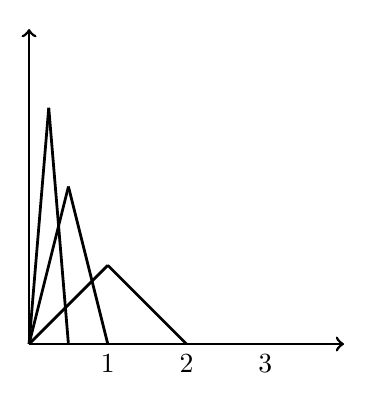
\begin{tikzpicture}[domain=1:5,line width=1pt]

\draw[->]  (0,0)  --  (0,4);
\draw[->]  (0,0)  --  (4,0);

\draw  (0,0)  --  (1,1);
\draw  (1,1)  --  (2,0);

\draw  (0,0)  --  (0.5,2);
\draw  (0.5,2)  --  (1,0);

\draw  (0,0)  --  (0.25,3);
\draw  (0.25,3)  --  (0.5,0);

\node [below] at (1,0) {1};
\node [below] at (2,0) {2};
\node [below] at (3,0) {3};

\end{tikzpicture}


$分析:x=0,f_n(x)\equiv 0$

$0<x \le 1时,\forall x(固定)当n>[\frac{2}{x}]时,f_n(x)=0$

$f(x)=\ntinf f_n(x)=0,\forall x \in [0,1]$

$\ntinf sup_{[0,1]}|f_n(x)-f(x)|=\ntinf |f_n(\frac{1}{n})|=\ntinf n=+\infty$

$\nl$

$例:设f_n(x)\rightrightarrows _{[a,b]} f(x),f_n(x)在[a,b]上有界,n\in N,证明:\{f_n(x)\}在[a,b]上$

$一致有界,也就是\exists M>0:|f_n(x)|\le M,\forall n \in N,\forall x \in [a,b]$

$f_n(x)在[a,b]上有界,对固定n,有|f_n(x)| \le M_n,\forall x \in [a,b]$

$\{f_n(x)\}在[a,b]上有界,对固定x,有|f_n(x)| \le M_x,\forall n \in N$

$对\epsilon_0=1,\exists N \in N:|f_n(x)-f(x)|<1,\forall n>N,\forall x in[a,b]$

$取n=N+1,则有|f(x)|<1+|f_{N+1}(x)|\triangleq M_1$

$又有|f_n(x)|<1+|f(x)|<1+M_1 \triangleq M_2,\forall n>N,\forall x \in [a,b]$

$记M=max(|f_1(x)|,....|f_N(x)|,M_2)$

若条件改为f(x)有界,有何结论?

$\nl$

$M-判别法(book p72),\sum \frac{1}{nln^2n}积分判敛法$

$ln(1-\frac{a}{nln^2n})\le ln(1+\frac{x}{nln^2n}) \le ln(1+\frac{a}{nln^2n})\le -ln(1-\frac{a}{nln^2n})$

$\nl$

$D-判别法(book,page.75)特例①\{a_n\}单调趋向0,亦成立 ②\sum \beta_i有界,亦成立$

$\nl$

$A-判别法(book,page.74)|sinx|\sum|sin nx| \le |sinx|\frac{1}{|sin\frac{x}{2}|}=2|cos\frac{x}{2}|\le 2$

$通项是否趋于0是必要条件,利用求导求出反例的\{x_k\}或者$

$\ntinf sup_D|a_n(x)| \ge \ntinf a_n(f(n))=... \ge c$

$f(x)=\nsuminf \frac{sinnx}{n^3}在R上一致连续,且有连续导数$

$由|\frac{sinnx}{n^3}|\le \frac{1}{n^3},\sum \frac{1}{n^3} 收敛,u_n(x)=\frac{sinnx}{n^3}\in C(R)故连续$

$\nsuminf u_n'(x)=\frac{cosnnx}{n^2},|\frac{cosnnx}{n^2}| \le \frac{1}{n^2},\forall n \in N,\forall x \in R,故\sum u_n'(x)在R上一致收敛。$
\end{document}

